\chapter{Preparation}

\guidance{%
Principally, this chapter should \textbf{describe the work which was
undertaken before code was written}, hardware built or theories worked on. It
should \textbf{show how the project proposal was further refined and
clarified}, so that the Implementation stage could go smoothly rather than by
trial and error.\\
Throughout this chapter and indeed the whole dissertation, it is essential to
\textbf{demonstrate that a proper professional approach was employed}.\\
The nature of this chapter will vary greatly from one dissertation to another
but, underlining the professional approach, this chapter will very likely
include a \textbf{section headed “Requirements Analysis”} and
\textbf{incorporate other references to the techniques of Software
Engineering}.\\
The chapter will cite any \textbf{new programming languages and systems which
had to be learnt} and will \textbf{mention complicated theories or
algorithms} which required understanding.\\
It is essential to \textbf{declare the Starting Point} (see Section 7). This
states \textbf{any existing codebase or materials} that your project builds
on.  The text here \textbf{can commonly be identical to the text in your
proposal}, but it may \textbf{enlarge on it or report variations}. For
instance, the true starting point may have turned out to be different from
that declared in the proposal and \textbf{such discrepancies must be
explained}.
}

\prechapter{%
  Before commencing implementation of the project, careful consideration was
  given to planning it. Current solutions were explored, studied and evaluated
  against the aims described in Section~\ref{intro:aims}. The rest of this
  chapter will explain the initial set-up, elaborate on  related work and
  outline the project's starting point.
}

\section{Project Planning}

This project presents a unique idea and breaks new ground. As such, the
methodology had to suit and reflect the largely exploratory nature of the
process. A spiral software development model was chosen: think of an idea,
modify the model (of Coq proof-objects), implement and propogate the necessary
changes, evaluate the end-result and repeat. This allowed for experimentation
of ideas and flexibility of implementation strategies.

Git (\href{http://git-scm.com}{\texttt{git-scm.com}}) and GitHub
(\href{http://github.com/dc-mak}{\texttt{github.com/dc-mak}}) were invaluable
during the project, allowing for easy tracking, reverting, reviewing and
collaborating.  New features could be tested on new branches before being
merged in and a copy of the work was safely backed up in one more place. GitHub
extensions such as \href{https://travis-ci.org}{Travis-CI} (continous
integration) were added in later, as it became apparent that precisely
specified versioning, build-dependencies and automated tests were useful in
spotting errors early.

\section{Requirements Analysis}
Several components of this project needed to function correctly, both
individially and in conjuction for it to work. Separate parts for
modelling/translation (from Coq to the chosen model), displaying and
interacting (Neo4j/Cypher) and computation (Neo4j/Cypher plugins)
needed to be developed and brought together. Below is a list of required
features used throughout development to guide and provide context for
implementation decisions.

\begin{itemize}

  \item \textbf{Modelling}: The model should
  \begin{enumerate}[label=\textbf{M\arabic*},ref={M\arabic*}]

    \item\label{req:m1} include as much relevant data as possible. Here,
      relevant means useful to understanding a large library, but not so much
      so as to obfuscate any information or make learning how to use the
      project more difficult.

    \item\label{req:m2} be flexible to work with and easy to translate. One
      could imagine different front-ends for interacting with and computing
      data from the model.

    \item\label{req:m3} strike a balance between size and precomputing too much
      data. Figuring out which pieces of data can be reconstructed later and
      which are beneficial to compute during modelling will be a matter of
      experimentation and weighing up ease of implementation versus ease of
      later processing.

  \end{enumerate}

  \item \textbf{Interaction}: Interacting with the model should
  \begin{enumerate}[label=\textbf{I\arabic*},ref={I\arabic*}]

    \item\label{req:i1} primarily, allow users to understand the data. The
      following two points follow from this principal goal.

    \item\label{req:i2} support both graphical and textual modes of use. Small
      queries and novice users are likely to benefit from the presence of a
      well-designed GUI\@. However, larger queries requiring more computation
      and flexibility will benefit from a traditional, shell-like interface.

    \item\label{req:i3} be interactive and extensible. A static presentation of
      data, even in a GUI, would fail to make full use of graph-databases and
      the ability to query, in whatever way the user desires, information
      dynamically.

  \end{enumerate}

  \item \textbf {Computation}: Working with the model's data should
  \begin{enumerate}[label=\textbf{C\arabic*},ref={C\arabic*}]

    \item\label{req:c1} be enabled by a core library of good defaults. Certain,
      common functions should be ready `out-of-the-box' and provide users all
      they need to get started.

    \item\label{req:c2} allow the user to add their own functions. It is not
      possible to imagine and implement all the functionality users may desire
      and so a way to extend the project to suit their own needs would be of
      great use.

  \end{enumerate}


\end{itemize}

\section{Technologies Used}

Choice of implementation languages was, although an important decision, almost
completely dictated by the programs at the core of the project (Coq and Neo4j).

Coq and its plugins \textendash~specifically, dpdgraph, which was used as a
starting point for extracting information about Coq proof-objects from compiled
proof-scripts \textendash~are written in OCaml
(\href{http://ocaml.org}{\texttt{ocaml.org}}).  Since it almost always wiser to
work with and modify existing sytems (and more representative of real-world
work) and as a functional language, OCaml benefits from strong, static (and
inferred) type-system (allowing for easy experimentation, greater confidence in
correctness), sticking to it for other parts of the tools which need not
necessarily be in OCaml (e.g.\ the \texttt{dpd2} utility) was a welcome and
easy decision. OCaml has several other benefits too, such as
inductively-defined datatypes (useful for manipulating Coq constructs) and good
editing tools.

Similarly, Neo4j and its plugins are (usually) written in Java, but several
lanaguages are supported for the latter, both by Neo4j officially and by the
community. As will be explained in Subsection~\ref{subsec:neo4j}, Java
and R were found to be the most suitable for achieving this project's goals.

\section{Coq Proof-Assistant}

The Coq proof-assistant -- implemented in OCaml -- can be viewed as both 
a system of logic -- in which case it is a realisation of the \emph{Calculus of
Inductive Constructions} -- and as a \emph{dependently-typed} programming
language. Its power and development are therefore most-suited and often geared
towards \emph{large scale} developments.

On the logical side, Coq lays claim to projects such as the Four-Colour
Theorem~\cite{gonthier2008formal} (60,000 lines) and the aformentioned
\emph{Feit-Thompson} theorem (approximately 170,000 lines, 15,000
definitions and 4,200 theorems) are feats of modern software-engineering.

On the programming language side, Coq has served as the basis for many equally
fantastic projects. The \emph{CompCert Verified C
Compiler}~\cite{leroy2012compcert} demonstrates the practical applications of
theorem-proving and dependently-typed programming by implementing and proving
correct an optimising compiler for the C programming language.
\emph{DeepSpec}~\cite{pierce2016science}, a recently announced meta-project,
aims to integrate several large projects such as \emph{CertiKOS} (operating
system kernels, \emph{Kami} (hardware), \emph{Vellvm} (verifying LLVM) and many
more in the hopes to provide complete, \emph{end-to-end} verification of
real-world systems.

\section{Neo4j Database and the Cypher Language}

Neo4j is a graph database system implemented in Java. Traditional, relational
database theory and systems are designed with the goal of storing and
manipulating information in the form of \emph{tables}. As such, working with
highly interconnected data, such as social network graphs is best tackled with
the alternative approach of \emph{graph databases}.

Briefly, a (directed) \emph{graph} is defined as $G = (V, E)$ where $V$ is a set
of vertices or \emph{nodes} and $E \subseteq V \times V$ is a set of edges or
\emph{relationships} between two nodes. A \emph{graph database} is an OLTP
(online transaction processing, meaning operated upon live, as data is
processed) database management system with CRUD (create, read, update and delete)
operations acting on a graph data model. Relationships are therefore promoted to
first-class citizens and can be manipulated and analysed.

\subsection{Cypher: An Illustrated Example}

\emph{Cypher} features heavy use of pattern-matching in an ASCII-art inspired
syntax.  The following (slightly contrived but hopefully illuminating) example
in Listing~\ref{lst:cypherexample} illustrates some of the key strengths of
graph-based modelling using Cypher. 

Suppose we have a puppy named ``Cliff'' looking for the nearest and most
familiar children (for this example, a person under the age of six) to play
with.

To see how Cliff (indirectly) likes/knows this child, we bind \emph{path} to the
result of the \emph{shortestPath} query.  For the path itself, we start with a
node following this structure: \mintinline{cypher}{(var:label {attrib: val})}.
We then have a \emph{labeled, transitive} relationship (explicitly limiting our
search to paths of up to length four) expressed as an arrow with a label
\texttt{-[..]->}. As such, we can discard any paths with relationships we do not
want (e.g.\ \texttt{HATES}). 

To filter based on more complex logic (than possible by pattern-matching directly
on labels and attributes) we can express the requirement that the age of a dog by
the name of Cliff be less than or equal to two (and similarly for the age of the
child) in the \mintinline{cypher}{WHERE} clause.

Lastly, we return the path and order the results by proximity as a row of
results, renaming the column of the child's name to simply ``name''.

\begin{listing}[tb]%

\caption{Example Cypher Query}\label{lst:cypherexample}

  \begin{minted}{cypher}
  MATCH path = shortestPath(
    (puppy:dog {name: "Cliff"})-[:LIKES|:KNOWS*..4]->(child:person))
  WHERE puppy.age <= 2 AND child.age < 6
  RETURN path,
         child.name AS name,
  ORDER BY other.distance_from_clifford
  \end{minted}

\end{listing}

\section{Related Work}

Some existing tools offer part of the solutions.%

dpdgraph
(\href{http://github.com/Karmaki/coq-dpdgraph}{\texttt{github.com/Karmaki/coq-dpdgraph}})
is a tool which analyses dependencies between \emph{compiled} Coq proofs. As
such, desirable information about notation, tactics, definitions and the
relationship between a type and its constructors is lost.

Coqdep is a utility included with Coq which analyses dependencies \emph{at the
module level} by tracking {\tt Require} and {\tt Import} statements.

Coq SerAPI
(\href{http://github.com/ejgallego/coq-serapi}{\texttt{github.com/ejgallego/coq-serapi}})
is a work-in-progress library and communication protocol for Coq designed to
make low-level interaction with Coq easier, especially for IDEs. It has a
starting point for gathering some statistics of proof-objects in a project.

\begin{table}[p]
  \centering

  \begin{tabular*}{\textwidth}{@{\extracolsep{\fill}} rcccccccccc}

    \toprule

    & \rot{Source Code} & \rot{Hyperlinks} & \rot{Precise Kinds}
    & \rot{Constr. \& Types~~} % for vertical space after 'Types'
    & \rot{Type Sig.} & \rot{Module depend.} & \rot{Graphical rep.}
    & \rot{Interactivity} & \rot{Statistics} & \rot{Object depend.} \\

    \midrule

    Coqdoc    & \Y & \Y & \Y & \Y & \Y & \N & \N & \N & \N & \N \\
    Coqdep    & \N & \M & \N & \N & \N & \Y & \Y & \N & \N & \N \\
    CoqSerAPI & \N & \N & \N & \N & \N & \N & \N & \Y & \Y & \N \\
    dpdgraph  & \N & \N & \M & \N & \N & \N & \Y & \N & \N & \Y \\

    \bottomrule

  \end{tabular*}

  \medskip
  \Y\  Has feature \hfill \N\ Does not have feature \hfill \M\ Can be extended to support it

  \bigskip
  \caption{Comparison of Features}\label{table:features}

\end{table}

The features chosen for comparison reflect the strengths of each tool
considered.

Bundle with Coq, coqdoc produces \textbf{hyperlinked source code} meaning
details such as the \textbf{precise kinds} of a proof-object, the
\textbf{constructors of a type} and the \textbf{type signatures} are immediately
visible; hence those 5 dimensions were included.  Also include in a Coq system
is coqdep: a tool for modelling \textbf{module-level dependencies} that can
output a \texttt{dot} file to present it \textbf{graphically}.

Coq Serialised (S-expression) API is an \textbf{interactive} IDE communication
protocol with facilities for gathering some basic \textbf{statistics}. Here,
interactive is used to mean that information is not presented all at-once,
\emph{statically}, but can instead be queried dynamically at run-time. An
example of a static dispaly is Figure~\ref{fig:static}; it shows a medium-sized
Coq library as ouput by dpdgraph.

In principle, coqdep and dpdgraph can also support some degree of interactivity,
with support from other tools (which translate \texttt{dot} files to interactive
JavaScript), although this is rarely done.  What dpdgraph does do well is model
\textbf{object dependencies}, with some scope for distinguishing precise kinds
and displaying information graphically.

\section{Starting Point}

Both Coq and Neo4j have a rich eco-system of tools and libraries built for them.
Hence, it was worthwhile to examine the current landscape to determine the
software available and then use it as a starting point effectively.

\subsection{Coq}

Coq is a \emph{large} project, devloped by INRIA (France), and its size and
complexity are best experienced through detangling the source code for oneself.
Just for the implementation of the system (not including the standard library),
Coq features approximately 3 major ASTs, 6 transformations between them, 3000
visible types, 9000 APIs and 521 implementation files containing 228,000 lines
of dense, functional OCaml.

However, most of this massive project is sporadically (and tersely) documented.
Even after consulting the Coq developers' mailing-list, several hours were spent
browsing the source code to overcome the severe difficulties in understanding
the project. Prior familiarity with \emph{using} Coq (as an introduction to
tactical theorem-proving and dependently-typed programming) was not useful for
understanding the internals beyond context and how to compile and use programs
and libraries. However, it did serve as invaluable insight for designing the
data-model during the implementation phase.

\subsection{Existing Tools for Coq}\label{prep:coqtools}

A number of tools were studied to learn their approaches and analyse their
strengths and weakeness. A full, detailed comparison between all the tools
mentioned and this project will be presented later, during
the~\nameref{chapter:evaluation} chapter.  What follows is a brief overview of each tool
and the reason it was insufficient for the purposes of meeting the project aims
and requirements.

\subsubsection{Coqdoc}

Coqdoc is a documentation tool for Coq projects, includes as part of the Coq
system.. It can output to raw text, HTML, \LaTeX~and a few other formats.
Although it supports prettifying code with syntax highlighting and unicode
characters, its most relevant feature was its hyperlinking: potentially useful
for building dependency graphs.

However, the whole tool worked on an entirely \emph{lexical} level, with no
formal parsing, understanding or elaboration of the code structure. Some efforts
were made to modify its output into a useful format (e.g.\ comma-separated
values) for other tools; however these did not prove fruitful because
tokenisation cannot infer or preserve as much information as full compilation.
Hence, since it could not meet any of the modelling requirements
(completeness~\ref{req:m1}, flexibility~\ref{req:m2} and
size/precomputation~\ref{req:m3}) this approach was abandoned.

\subsubsection{Coqdep}
Coqdep is a tool which computes inter-module dependencies for Coq and
OCaml programs, outputtting in a format readable by the \texttt{make} program.
Although on first impressions, this tool seemed to offer more flexibility than
coqdoc, it was even more restrictive: it simply searches for keywords (such as
\texttt{Require} or \texttt{Import} for Coq  and \texttt{open} or dot-notation
module usage for OCaml) per file and outputs them accordingly.  As with coqdoc
(and for the same reasons), this approach was also abandoned.

\subsubsection{CoqSerAPI}

\emph{Coq Serialized (S-expression) API} is a new library and communication protocol
aiming to make low-level interactions easier (using OCaml datatypes and
s-expressions), particularly for tool/IDE developers. While this is likely to
be useful in the future, it is still far from complete and is more geared
towards interactive \emph{construction} (via a tool/IDE) rather than
\emph{analysis}. As such, tracking dependencies (critical to the modelling
requirements) is not possible.

\subsubsection{dpdgraph}

dpdgraph is a tool which extracts dependencies between Coq objects from compiled
Coq object-files to a \texttt{.dpd} file. It includes two example tools:
\texttt{dpd2dot} (for producing a \texttt{.dot} file for static visualisation)
and \texttt{dpdusage} (for finding unused definitions). Its developers intended
it to be a starting point for tools to build upon.

Although lots of information such as notation, the relationship between
constructors and the types they construct, proof tactics, the precise kind of an
object (e.g.\  fixpoint, class, lemma, theorem, etc.) and which module an object
belongs to was missing, it seemed unlikely that the information was not present
in the compiled object files. Assuming that the data was already present in
those files, but simply \emph{ignored or unused}, implementation of the
modelling aspect of this project focused on understanding and augmenting
dpdgraph to add the missing pieces to the model and convert the whole thing to
comma-separated values (henceforth referred to as CSVs)

\subsection{Neo4j}\label{subsec:neo4j}

Neo4j is one of the most popular graph database systems. It supports both
graphical and textual modes of use and is easily extensible (through Cypher
plugins and several language-specific bindings and libraries). It meets all the
interaction requirement of helping users to understand data, being flexible in
its use and extensible in its capabilities. It even includes a tool to import
CSVs files containing nodes and edges into a new database, which meant modelling
could be focused towards extracting and expressing in a simple format as much
information as possible.

Neo4j also includes an interactive graphical interface, accessible through an
ordinary web-browser. As can be seen on Figure~\ref{fig:neo4jbrowser}, the tool
offers 
\begin{itemize}
  \item an overview of the current labels, relationships and properties in the
        database
  \item syntax-highlighted interactive-editing box
  \item graphical representation of query result (with options to view it as
        rows like a shell, or raw JSON text results) with profiling information
        along the bottom
  \item easy access to favourite queries and scripts (the star on the left)
  \item easy access to documentation and system information (the book on the
        left)
  \item and many more features such as browser sync, settings and the `about'
        section.
\end{itemize}

\begin{figure}[tbp]

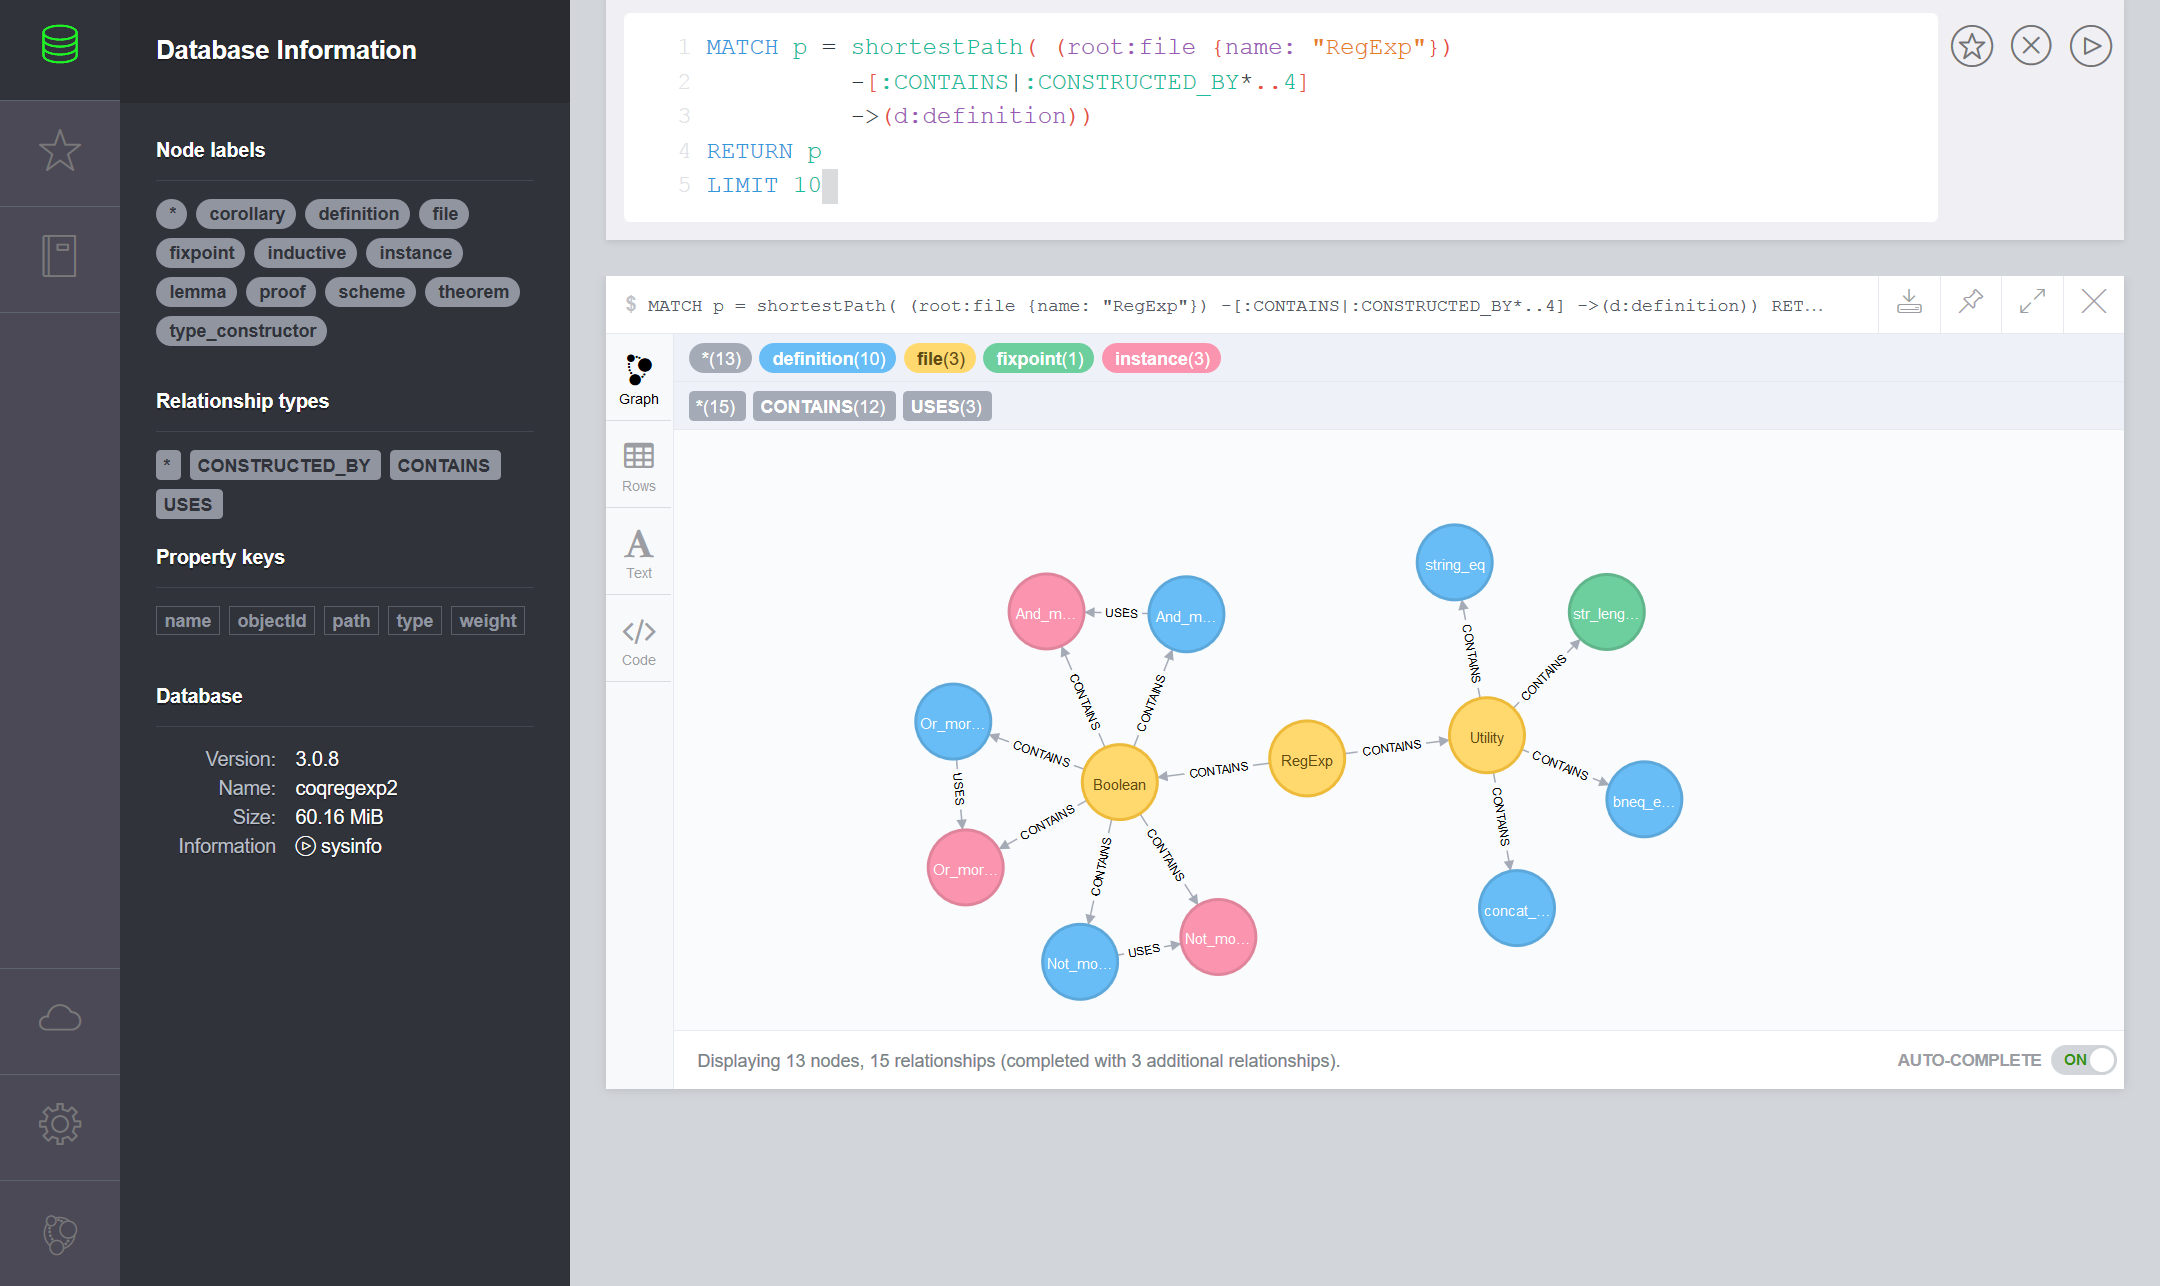
\includegraphics[width=\textwidth]{img/Neo4j_Browser.png}
\caption{Neo4j Interactive Browser}\label{fig:neo4jbrowser}

\end{figure}

\subsection{Existing Tools for Neo4j}\label{subsec:existtoolsneo4j}

Neo4j features rich-integration with many languages, libraries and tools.
Of those, the following were the most relevant and useful tools for meeting
the project requirements.

\subsubsection{APOC: Awesome Procedures on Cypher}

\href{http://github.com/neo4j-contrib/neo4j-apoc-procedures}{\emph{Awesome
Procedures on Cypher}, or \emph{APOC}} for short, is a community-maintained Java
plugin featuring several graph algorithms callable from within Cypher itself.
Although there are other extension libraries (such as MazeRunner), APOC is well
documented, up-to-date and the most comprehensive, and therefore the obvious
choice as a foundation. By being a Java library hooked into Cypher, it offered
the potential for additional functionality to be built on top of it which
packaged-up some of the more complex features into \emph{domain-specific}
queries, intended for Coq users not familiar with Neo4j to get started with.
Thus, APOC helps step towards meeting the \emph{interaction} requirements for
this project by being easy to understand, flexibile to use and extensible; even
going part-way towards meeting the \emph{computation} requirements.

\subsubsection{igraph}\label{subsubsec:neo4jtoolsigraph}

APOC has some key strengths that made it a good choice: it is easy to install
and use and has some basic graph algorithms to get started with.  However, its
main focus is on interacting with and combining different sorts and sources of
data and so lacks graph analysis functionality \emph{beyond} the basics. The
fact that it is implemented in Java further adds to its limitations: it is not
well-suited to more intense analyses over large graphs of libaries and is
insufficient to \emph{fully} meet the \emph{computation} requirements of this
project.

For such tasks, \href{http://www.igraph.org}{igraph} is ideal: it is described
on its website as a \emph{collection of network analysis tools, with the
emphasis on efficiency, portability and ease of use}. Written in C/C++ (with
bindings for R and Python), igraph offers a \emph{comprehensive} set of graph
algorithms without sacrificing on performance. These alogrithms and their uses
will be described later, in the Implementation chapter. For now, it suffices to
surmise that although igraph is not as easy to interact with (via the
statistics-oriented programming language R, as detailed in the next paragraph)
as APOC, the extra capabilities afforded were indispensible towards achieving
the \emph{computation} requirements of a core library of good defaults.

\subsubsection{visNetwork}

With igraph and APOC providing starting points for the computational aspects of
the projects, and the interactive Neo4j browser providing a well-polished,
graphical mode of interaction with basic, but useful, visualisation, the last
piece of the project was to incorporate the extra information gained from
\emph{executing} the graph algorithms.

\emph{Several} visualisation programs exist for Neo4j; however, many are for
commercial, industrial use and offer the features/complexity (and pricing) to
match. All tools which offer live visualisation with built-in Cypher query
execution (e.g. KeyLines, TomSawyer, Linkurious) are proprietary, requiring a
fee to use and offering more granularity than required. Offline (and
open-source) solutions (which require data to be exported in some manner before
visualisation) such as Gephi or Alchemy.js offer similarly many features, but at
the cost of a steep learning curve.  Ultimately,
\href{http://datastorm-open.github.io/visNetwork}{visNetwork}, (an R library
exporting to JavaScript which can be rendered inside a browser) was chosen due
to its simplicity and ease of integration with previous tools mentioned above.

As stated previously, igraph provides a comprehensive set of graph algorithms
with an \emph{emphasis on efficiency, portability and ease of use}.  The
metrics these algorithms compute and an interpretation of them in the context
of mathematical theories is given next.  Although a wealth of algorithms are
available in igraph, visualisation and evaluation was focused on only the most
common and well-known ones.

\subsubsection{Centrality}

\emph{Centrality} measures offer a way to characterise a node's
\emph{importance}.

\textbf{Betweenness} centrality is a measure based on shortest paths. For each
node ($v$), the number of shortest paths ($\sigma_{st}$) which pass through it
($\sigma_{st}\left(v\right)$) is its betweenness centrality. When applied to
mathematical theories, how ``unavoidable'' a given object is for the results
which mention it.~\cite{freeman1977}

\begin{equation}
  g\left(v\right) = \sum_{s \neq v \neq t} \frac{\sigma_{st}\left(v\right)}{\sigma_{st}}
\end{equation}

\textbf{Closeness} centrality is also measure based on shortest paths. For each
node, the sum of the length of all shortest paths to every other node is its
closeness centrality. In a directed, dependency graph of mathematical theories,
this corresponds to how ``foundational'' a node is. It is typically calculated
as the reciprocal of \emph{farness} ($\sum_{y}d\left(y,x\right)$), scaled by
the number of nodes in the graph ($N$) to allow comparisons with graphs of
different sizes.~\cite{bavelas1950}

\begin{equation}
  C\left(x\right) = \frac{N}{\sum_{y}d\left(y,x\right)}
\end{equation}

\textbf{PageRank} is a variant of \textbf{eigenvector} centrality.  For an
adjacency matrix $\mathbf{A}$, the v\textsuperscript{th} component of the
eigenvector $\mathbf{x}$ (whose entries must all be non-negative, corresponding
to the greatest eigenvalue $\lambda$) is the v\textsuperscript{th} node's
\emph{relative, eigenvector} centrality. Normalising the eigenvector provides
the \emph{absolute eigenvector} centralities.~\cite{newman2008}

The principle behind such a measure is that connections to high-ranking nodes
contribute more to a node's rank than connections to low-ranking nodes.  As
such, for mathematical theories, it is like a \emph{weighted
in-degree/number-of-uses} which takes into account the importance of the nodes
which is using a given type, proof or defintion.

PageRank is similar; instead of the vector $\mathbf{x}$ such that $\mathbf{Ax}
= \lambda\mathbf{x}$, for number of nodes $N$, random-jump probability $1-d$,
stochastic adjacency matrix $\mathbf{L}$, we want $\mathbf{r}$ which satisfies
equation~\ref{eqn:pagerank}.~\cite{page1999} Hence, it can be viewed as the a
probability of an easily-confused, randomly-perusing mathematician coming
across a given proof or definition, perhaps upon a first reading.

\begin{equation}~\label{eqn:pagerank}
  \mathbf{r} = \frac{\left(1-d\right)}{N} \mathbf{1} + d\mathbf{Lr}
\end{equation}

\subsubsection{Community Detection}

Complex networks can exhibit community structure; that is, the graph can be
(roughly) divided into sparsely-connected dense groups. Although mathematical
theories are often divided into sections, chapters and books, the following
algorithms provide scope for re-evaluating these groupings.

\textbf{Label propagation} is a simple, near linear time method for
determining which community a node belongs to. Each node starts with a unique
label, after which, on successive iterations, it adopts the label held by most
of its neighbours, until a consensus is reached. This whole procedure is
repeated a few times and an aggregate result constitutes the
output.~\cite{raghavan2007}

\textbf{Edge betweenness} (like betweenness centrality), is also based on
shortest paths, with the idea that edges separating communities are likely to
have high edge betweenness (since all shortest paths must pass through them).
Removing the edge with the greatest betweenness value and recomputing over the
remaining edges successively will result in a rooted tree, a hierarchical map
(called a dendrogram) where the root represents the whole graph and the leaves
represent individual nodes.~\cite{newman2004}

\textbf{Modularity} is a measure of how well network can be divided.
Formally, it is the fraction of edges that fall within a given grouping
(across the whole graph) minus the expected number of those which could have
fallen within the group by chance (and so is a real number between $-0.5$ and
$1$). Calculating this in an optimal manner is an NP-complete problem, and so
a fast and greedy version of it was used.~\cite{clauset2004}


\subsubsection{R}

\href{http://www.r-project.org}{R is a statistics-oriented programming language},
part of the Free Software Foundation's GNU poject. It is relevant for this
project because it offers an easy way to tie together Neo4j (through official
bindings), igraph and visualisation using visNetwork. This convenience came at
the price of having to learn R for this project, having been unfamiliar with it
prior. Nonetheless, it is a well-documented, relatively easy to pick-up language
and offered even more opportunities for learning during the course of this
project.

\section{Summary}

A detailed account into the planning of this project was given. The choice of
development methodology (spiral) and development tools (Git, GitHub, Travis-CI)
were noted. Requirements on modelling, interaction and computation were
explained and the choice of technologies and tools used as statrting points
(Coq, OCaml, dpdgraph, Neo4j, APOC, igraph, R and visNetwork) were justified
\emph{in relation} to \emph{which} requirements they satisfied.
